\documentclass[legalpaper]{article}
\usepackage[legalpaper, margin=1in]{geometry}
\usepackage[T1]{fontenc}
\usepackage[utf8]{inputenc}
\usepackage[italian]{babel}
\usepackage{graphicx}
\begin{document}


\title{%
\raggedright \textbf{Progetto Basi di Dati} \\ \large \bigskip Progettazione ed implementazione di una base di dati relazionale per la gestione delle assistenze di una ditta di gestione di impianti di riscaldamento.}
\maketitle

\begin{flushleft}
\author{Brugnera Matteo 137370 \and \\ Parata Loris 144338 \and \\ Giovanni Rasera 143395}

\end{flushleft}

\newpage

\tableofcontents

\newpage
\section{Introduzione}
\rule{\linewidth}{1.5pt}
\subsection{Introduzione}
Lo scopo del progetto è quello di implementare un sistema informativo, nello specifico una base di dati relazionale, in grado di gestire le prestazioni di un centro di assistenza per impianti di riscaldamento. 
Le funzionalità che dovrà prevedere il sistema sono di seguito specificate.
L'azienda deve permettere di gestire le richieste di assitenza, che sono a loro volta composte un insieme di interventi effettuati da tecnici specializzati.
I servizi offerti sono usufruibili solo da clienti facenti parte di due tipologie di persone giuridiche, che rappresentano aziende ed enti pubblici, o persone fisiche che rappresentano i singoli cittadini.
Ognuno di essi avrà un codice identificativo generato dal sistema una volta divenuti clienti, grazie al quale si potrà risalire a tutti i loro dati. 
In particolare, per le aziende e gli enti pubblici si vuole tenere codice di Partita IVA, mentre per i singoli cittadini il Codice Fiscale.
Le assistenze vengono identificate univocamente dal codice di Assistenza. Ogni intervento è legato all'assistenza ed identificato univocamente da un numero progressivo. 
Le richieste di assistenza vengono accettate solamente se la tipologia di problematica è presente nella lista di problematiche risolvibili. \\
Per ogni intervento, si tiene traccia di:
\medskip
\begin{itemize}
    \item cliente richiedente l'assistenza;
    \item tipologia del sistema e del guasto;
    \item tecnico assegnato;
    \item intervento di riferimento;
    \item data intervento;
    \item durata intervento.
\end{itemize}


\newpage
\section{Raccolta e analisi dei requisiti}
\rule{\linewidth}{1.5pt}
\subsection{Tabella dei requisiti}
Questa fase rappresenta l’inizio della realizzazione di un sistema informativo. Con essa si cerca di comprendere quali sono gli obiettivi che vengono richiesti. 
È necessario porre particolare attenzione alla terminologia utilizzata, in modo tale da poter procedere alla formulazione dei requisiti.

\subsection{Glossario dei termini}
Il linguaggio naturale è ambiguo ecco perchè è necessario chiarire con precisione ogni termine utilizzato durante questa fase di progettazione.
Per ogni termine introdotto si definiscono:
\begin{itemize}
    \item Descrizione : definizione semantica del termine
    \item Sinonimi: eventuali sinonimi utilizzati per identificare lo stesso oggetto
    \item Correlazioni: le relazioni esistenti tra i diversi oggetti
\end{itemize}
\medskip
Il seguente glossario definisce i termini più rilevanti che saranno l’input della fase di progettazione concettuale.
\medskip

\begin{tabular}{ |p{1.5cm}|p{8cm}|p{3cm}|p{2.5cm}| }
\hline
\multicolumn{4}{|c|}{\textbf{Glossario}} \\
\hline
\textbf{Termine} & \textbf{Descrizione} & \textbf{Sinonimo} & \textbf{Correlazione} \\
\hline
Cliente &  soggetto che effettua una richiesta di assistenza all'azienda & Persona Giuridica \newline Persona fisica & Assistenza \newline Guasto \\ \hline

Persona fisica &  persona fisica che rappresenta se stesso e che effettuera' una richiesta di assistenza all'azienda di assistenza &  Singolo cittadino \newline Cliente &  Cliente \\ \hline

Persona giuridica &  persona fisica che rappresenta un'azienda o un ente pubblico che effettuera' una richiesta di assistenza all'azienda di assistenza & Azienda \newline Ente Pubblico \newline Cliente &  Cliente \\ \hline

Assistenza & inizializzazione di un nuovo contratto di assistenza tra un cliente e l'azienda di assistenza, ogni assistenza composta da almeno un intervento   &  & Cliente \newline Intervento \newline Guasto \\ \hline

Intervento & prestazione eseguita da un tecnico per risolvere un guasto & Prestazione & Guasto \newline Tecnico \newline Guasto \\ \hline

Tecnico  & dipendente specializzato dell'azienda di assistenza, specializzato nella risoluzione di guasti di un sistema specifico & Dipendente & Guasto \newline Intervento \\ \hline

Guasto  & problematica di un'sistema specifico e di una specifica tipologia  & Problema &  Tecnico  \newline Cliente \newline Assistenza \\ \hline

\end{tabular}


\subsection{Riscrittura dei requisiti}
In questa fase vengono tradotte le richieste della consegna in requisiti da soddisfare e viene definito il ruolo delle entità all’interno della base di dati.
\newline

\begin{tabular}{ |p{16 cm}| }
\hline
\multicolumn{1}{|c|}{\textbf{Riscrittura dei requisiti}} \\
\hline
\textbf{Frasi di natura generale}  \\
\hline
- Si vuole implementare un sistema automatico per la gestione dei servizi di assistenza e dei relativi interventi di un'azienda d'assistenza di impianti di riscaldamento \newline
- Le assistenze possono essere richieste solamente per problemi risolvibili dai tecnici dell'azienda.\\ \hline
\textbf{Frasi relative al cliente}  \\
\hline
-  I clienti possono essere di diversa natura:  \newline persone giuridiche, che comprende aziende ed enti pubblici; \newline  singoli cittadini (persone fisiche). \newline
- I clienti richiedono un'assistenza relativa ad un guasto specifico di un sistema specifico.\\
\hline
\textbf{Frasi relative all'assistenza}  \\
\hline
- Un'assistenza è caratterizzata da un codice identificativo generato dal sistema. Nel momento in cui viene completata l'assitenza viene memorizzato il giorno di fine di assitenza\\
\hline
\textbf{Frasi relative all'intervento}  \\
\hline
- Un intervento è identificato da un numero progressivo riferito all'assistenza di appartenenza. Inoltre, è caratterizzato dalla modalità con la quale può essere eseguito (da remoto o in sede), dalla data e dalla relativa durata del singolo intervento misurato in ore (0-24). Un solo intervento può essere eseguito durante la giornata lavorativa.\\
\hline
\textbf{Frasi relative al tecnico}  \\
\hline
- Un tecnico è identificato dal suo codice fiscale, dai suoi dati anagrafici, un recapito telefonico ed un email, una data di assunzione e indirizzo del domicilio.\\
\hline
\textbf{Frasi relative al guasto}  \\
\hline
- Un guasto è rappresentato dalla combinazione tra sistema e tipologia di problema.\\
\hline
\textbf{Frasi relative al coinvolgimento di cliente, assistenza e guasto}  \\
\hline
- Quando un cliente richiede un'assistenza relativa ad uno specifico guasto, per poter finalizzare e registrare la data di inizio assistenza è necessario che sia presente quella tipologia di guasto tra i guasti riparabili per quel sistema.\\
\hline
\textbf{Frasi relative al coinvolgimento di tecnico e guasto}  \\
\hline
- Un tecnico può essere assunto se è capace di risolvere almeno una tipologia di guasti per un determinato sistema, ma nel tempo può ampliare le proprie competenze e risolvere problemi anche di tipologia diversa e sistemi diversi.\\
\hline


\textbf{Frasi relative al coinvolgimento di assistenza, intervento, tecnico e guasto}  \\
\hline
- Una volta effettuata la richiesta di assistenza, si pianifica il primo intervento assegnando un tecnico competente per risolvere quel tipo di guasto, controllando che in quella data non ci sia un intervento programmato per lo stesso tecnico altrove.\\
\hline
\end{tabular}

\subsection{Caso di studio} 
	Per la realizzazione del sistema informativo è stato teorizzato un business-plan di un'azienda di piccole/medie dimensioni che opera a livello regionale.
	Consideriamo la seguente situazione dopo 10 anni di attività:
	\begin{itemize}
		\item numero clienti totale: 10000 (fedeli e non);
		\item numero tecnici totali: 75;
		\item media clienti annuali: 1000;
		\item media di 2 richieste di assistenza per cliente all'anno;
		\item media di 3 interventi per ogni assistenza richiesta;
		\item in media 300 clienti rimangono fedeli al nostro servizio;
		\textbf{NB: DEVI INSERIRE LA DEFINIZIONE DI FEDELI NELLA TABELLA DEI TERMINI !!!!!!! ---> per fedeli si intende tutti quei clienti che faranno rifermento a noi come aziende per qualsiasi guasto negli anni a venire}
	\end{itemize}
	Supponiamo che dei 10000 clienti avuti in 10 anni, 300 siano rimasti fedeli a noi. Di conseguenza l'undicesimo anno operativo dell'azienda otterrà 3000+1000=4000 clienti (fedeli + nuovi clienti annuali, fedeli e non). Facendo così, avremo 4000*2=8000 assistenze totali  e quindi ciò implica 24000 interventi.\\
	Quest'ultimi vengono divisi tra i 75 tecnici, facendo sì che ognuno di essi abbia in media 320 interventi da eseguire in un anno.\\
	Nel dodicesimo anno otteniamo un totale di 3300 clienti fedeli, arrivando a fine anno con 4300 clienti e 25800 interventi fatti, ovvero 344 a tecnico. Tutto ciò risulta essere troppo oppressivo per un lavoratore, quindi dobbiamo aumentare il numero di tecnici da assumere a fronte dell'aumento della clientela, aumentando così il volume dell'azienda stessa.\\
	Se supponiamo che ogni anno vengono assunti e/o formati 6 nuovi dipendenti, abbiamo che il rapporto interventi/tecnici rimane sempre intorno ai 320 (ovvero ogni tecnico avrà 320 interventi all'anno).\\
	Ad esempio il tredicesimo anno avremmo 87 operai con 27.600 interventi, cioè intorno ai 317 interventi per operaio.\\
	Ultimo appunto importante riguarda la distinzione che è possibile fare tra i vari clienti.
	Più in particolare del 100\% dei clienti, il 50\% risulta essere un ente pubblico mentre il restante 50\% è privato. Del 50\% pubblico, il suo 70\% fa riferimento alle aziende, mentre il 30\% agli enti pubblici.
	
	\subsection{Requisiti operazionali (NB da inserire nel capitolo 2.5!!!!!!!!!!!!!!!!!!!)}
	Le operazioni principali che prenderemo in considerazione sono:
	\begin{itemize}
		\item operazione 1: inserire un nuovo cliente -> 19 volte a settimana;
		\item operazione 2: creare una richiesta di assistenza -> 150 volte a settimana;
		\item operazione 3: creare una richiesta di intervento -> 450 volte a settimana;
		\item operazione 4: inserire un nuovo dipendente -> 6 all'anno;
		\item operazione 5: visualizzare le richieste di assistenza di uno specifico cliente -> 30 a settimana;
		\item operazione 6: visualizzare il numero di guasti per tipologia -> 1 a settimana. Questo dato può fornirci utili informazioni inerenti alle tipologie di sistemi meno affidabili; 
		\item operazione 7: visualizzare quale tecnico ha eseguito il maggior numero di interventi e la durata complessiva -> 1 volta al mese. Questo dato può essere utilizzato per vedere in quali reparti ci sono carenze di tecnici, andando così a mirare l'assunzione/training dei nuovi dipendenti;
		\item operazione 8: visualizzare lo storico degli interventi di un assistenza -> 10 volte al giorno, perchè si vuole monitorare il più possibile l'impiego dei tecnici, cioè chi è impegnato e dove;
		\item operazione 9: visualizzare il tempo complessivo degli interventi per ogni cliente -> 1 volta a settimana per i soli clienti che hanno richiesto un'assistenza nel periodo immediato;
		\item operazione 10: visualizzare gli interventi effettuati da ogni tecnico -> 3 volte a settimana;
	\end{itemize}

\subsection{Requisiti operazionali}
Le operazioni principali che verranno sviluppate sono:
\begin{itemize}
    \item Operazione 1: inserire un nuovo cliente ( circa 2 volte a settimana)
    \item Operazione 2: creare una richiesta di assistenza, 40 a settimana
    \item Operazione 3: creare una richiesta di intervento, 120 a settimana
    \item Operazione 4: inserire un nuovo dipendente, 6 all' anno
    \item Operazione 5: visualizzare le richieste di assistenza di uno specifico cliente, 20 a settimana
    \item Operazione 6: visualizzare il numero di guasti per tipologia, 1 a settimana
    \item Operazione 7: visualizzare quale tecnico ha eseguito il maggior numero di interventi e la durata complessiva, 1 volta al mese
    \item Operazione 8: visualizzare lo storico degli interventi di un assistenza, 10 volte al giorno
    \item Operazione 9: visualizzare il tempo complessivo degli interventi per ogni cliente, 1 volta al mese per ogni cliente che ha richiesto un'assistenza.
    \item Operazione 10: visualizzare gli interventi effettuati da ogni tecnico, 1 volta alla settimana.
\end{itemize}


\newpage
\section{Progettazione concettuale}
\rule{\linewidth}{1.5pt}

\subsection{Definizione specifiche}
Per scrivere il nostro schema e per descrivere le specifiche e realizzare la relazione abbiamo utilizzato questa convenzione:
\begin{itemize}
	\item Entità: prima lettera MAIUSCOLA e il resto minuscolo\\
	Esempio: Assistenza, Cliente, Intervento.
	\item Relazione: tutta la parola minuscola\\
	Esempio: è capace di risolvere, composta da.
	\item Attibuti delle entità e delle relazioni: prima lettera minuscola e il resto della parola cammellizzato\\
	Esempio: dataFineAssistenza, numeroIntervento, dataAssunzione.
	\item Rappresentazione di un attributo di un entità o di una relazione: utilizzato il simbolo      ->      tra l'entità e l'attributo\\
	Esempio: Entità->attributoUno, Entità->attributoDue, Intervento->modalità.
\end{itemize}
\newpage
\subsection{Schema Entità-Relazione}
Il modello Entità-Relazione (E-R) è il modello teorico utilizzato in questa fase di progettazione concettuale per la rappresentazione grafica e concettuale dello scenario di interesse. Questo permette di comprendere in modo semplice ed intuitivo quali sono i soggetti principali della scena e come sono relazionati tra di loro. 
Modello E-R dell'azienda di assistenza:
\newline

\begin{figure}[ht]
	\centering
	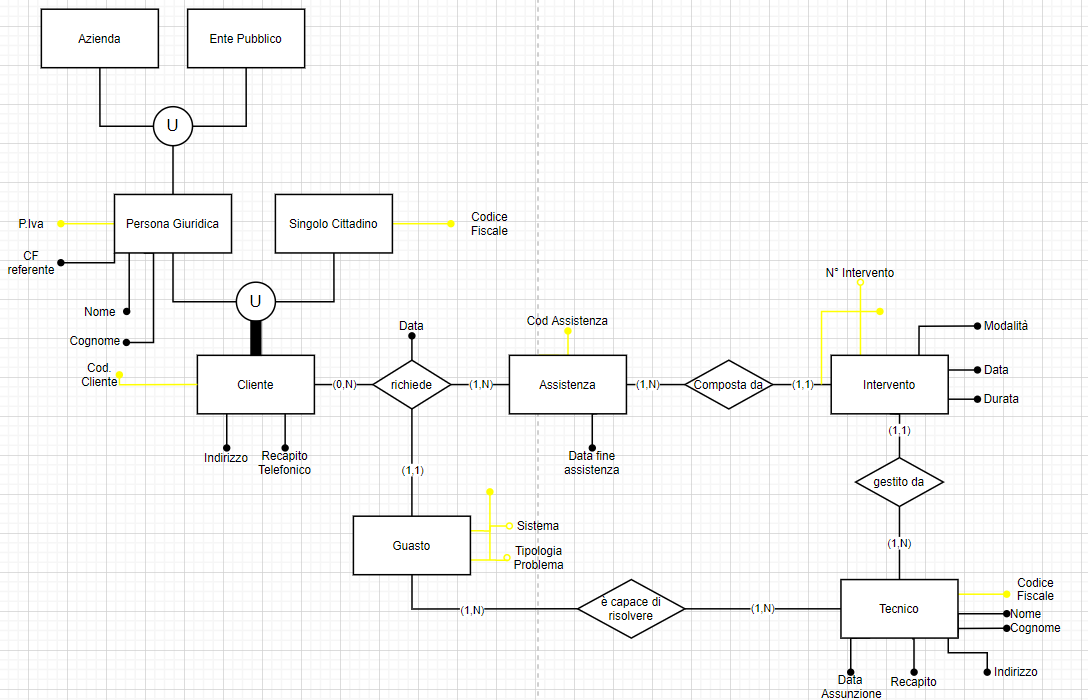
\includegraphics[width=0.7\linewidth]{../Parata/ER_prototipo_v2}
	\caption[]{Schema E/R complessivo}
	\label{fig:erprototipov2}
\end{figure}


\subsubsection{Evidenziazione dello schema E-R}



\begin{figure}[!ht]
	\centering
	\begin{minipage}[b]{0.4\textwidth}
		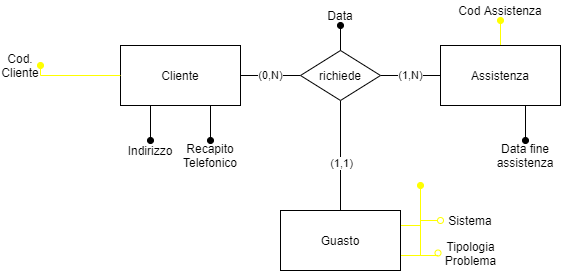
\includegraphics[width=\linewidth]{../Parata/relazione_livello_superiore}
			\caption{Relazione di livello superiore al secondo}
		\label{fig:relazionelivellosuperiore}

	\end{minipage}
\hfill
	\begin{minipage}[b]{0.4\textwidth}
		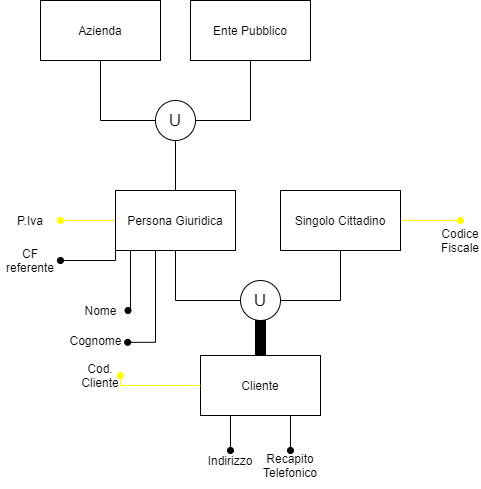
\includegraphics[width=\linewidth]{../Parata/generalizzazione_diagram}
		\caption{Generalizzazione}
		\label{fig:generalizzazionediagram}
	\end{minipage}
\end{figure}
\paragraph{Figura 2}
lo schema mette in evidenza la presenza di una relazione ternaria tra le entità Cliente, Guasto ed Assistenza.
\paragraph{Figura 3}
lo schema mette in evidenza la presenza di una generalizzazione parziale esclusiva tra le entità Azienda ed Ente Pubblico, le due entità che rappresentano due concetti diversi. Ma nel contempo sono rappresentati da una Persona Giuridica per legge.
\paragraph{Figura 4} Lo schema mette in evidenza la presenza di una generalizzazione esclusiva totale tra le entità Persona Giuridica e Singolo Cittadino che differiscono per codice identificativo univoco legalmente. Una Persona Giuridica viene distinta tramite Partita Iva, mentre un Singolo Cittadino dal proprio CodiceFiscale.
\newpage
\subsection{Regole di derivazione}


\subsection{Vincoli d'integrità}
I vincoli d'integrità sono tutte le proprietà di una base-di-dati, sono esprimibili 
tramite dei predicati; questi devono essere veri per garantire la validità dello schema.\\
\newline
Di seguito sono riportati i vincoli d'integrità presenti nel modello E-R:
\begin{itemize}
	\item L'attributo Assistenza->dataFineAssistenza deve essere maggiore o uguale\\ della proprietà richiede->data.
	\item Se Assistenza->dataFineAssistenza non è NULL allora: il numero di Interventi appartenenti a un'Assistenza deve essere minore o uguale alla differenza (in giorni) tra \\richiede->data e Assistenza->dataFineAssistenza.\\Questo vincolo deriva dal fatto che è possibile fare un Intervento al giorno per singola Assistenza.
	\item L'attributo Intervento->durata deve essere un valore nel dominio (0, 24).
	Il valore della durata è rappresentato tramite il sistema orario a 24 ore.
	\item Un Tecnico non deve essere assegnato a degli Interventi diversi nello stesso giorno.
	
\end{itemize}

\subsection{Pattern di progettazione}
I pattern di progetto sono delle soluzioni progettuali a problemi comuni. Si elencano di seguito i pattern più utilizzati nella progettazione concettuale in basi di dati, applicati allo schema concettuale illustrato precedentemente:
\begin{itemize}
	\item Relazione "parte-di":\\
	- Un'assitenza è composta da diversi interventi
	
	\item Semplificazione di reificazione di relazione ternaria\\
	– Utilizzata per distinguere le richieste di Assistenza che effettua un determinato Cliente inerente ad un determinato Guasto. 
	

\end{itemize}
	

\newpage
\section{Progettazione logica}
\rule{\linewidth}{1.5pt}
	\section{Progettazione logica}
		Lo scopo della progettazione logica è di costruire uno schema relazionale che rappresenti in modo accurato, efficiente e soprattutto correttamente tutte le informazioni descritte da uno schema ER prodotto durante la fase precedente. \\
		Questo non è una semplice trasformazione da un modello ad un altro per due motivi:
		\begin{itemize}
			\item non tutti i costrutti del modello ER possono essere tradotti nel modello relazionale;
			\item lo schema deve essere ristrutturato in modo che l'esecuzione delle operazioni avvenga il più efficientemente possibile
		\end{itemize}
		Inoltre si controllano e governano le ridondanze. Infatti per analizzarle si usano: 
		\begin{itemize}
			\item i volumi dei dati;
			\item operazioni attese;
			\item frequenza delle operazioni;
		\end{itemize}
		\'E utile dividere questo tipo di progettazione in due semplici step:
		\begin{itemize}
			\item ristrutturazione dello schema ER, basato sull'ottimizzazione e semplificazione dello schema;
			\item traduzione nel modello logico.
		\end{itemize}
		\begin{figure}[ht]
			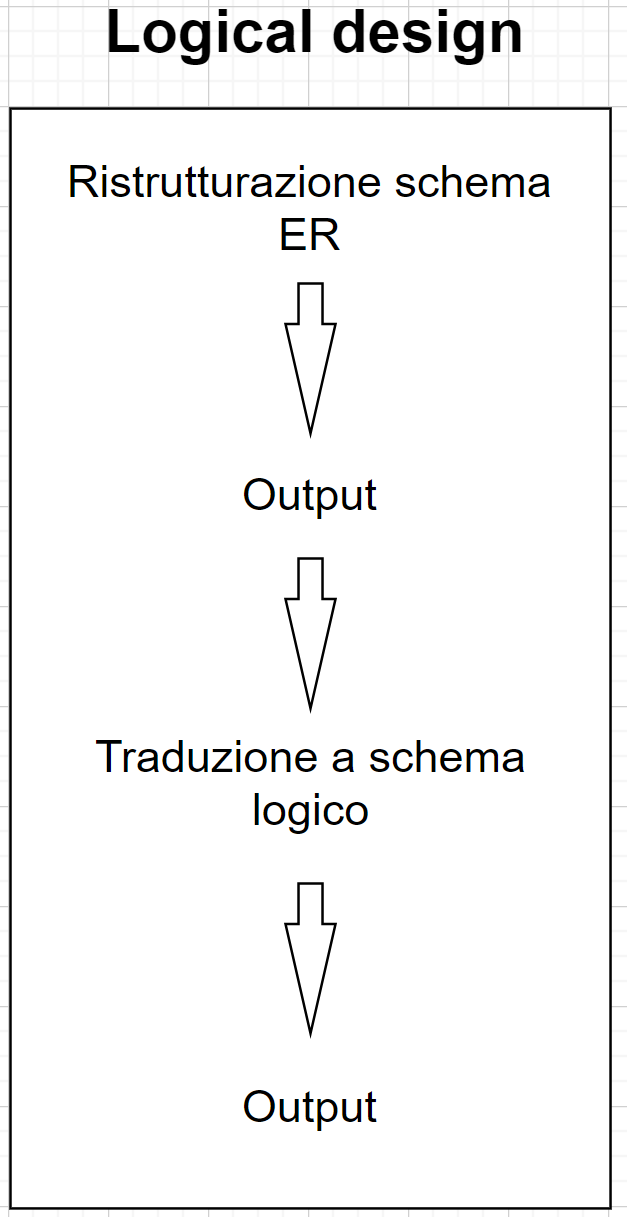
\includegraphics[width=4cm]{../Parata/Schema Prog. Logica}
		\end{figure}
	\subsection{Tabella dei volumi}
		In questa sezione andiamo a definire il numero di occorrenze per ogni entità e relazione presente all'interno dello schema ER. Viene ipotizzato che i volumi facciano riferimento all'attività dopo i suoi dieci anni di vita.\\
		\newline
		\renewcommand\arraystretch{2}
		\begin{tabular}{ |p{5cm}|p{2cm}|p{5cm}| }
			\hline
			\multicolumn{3}{|c|}{\textbf{Tabella dei volumi}} \\
			\hline
			\textbf{Entità/Relazione} & \textbf{Tipo} & \textbf{Volume} \\
			\hline
			Azienda & E & 700 \\ \hline
			Ente Pubblico & E & 300 \\ \hline
			Persona Giuridica & E & 1000 \\ \hline
			Singolo Cittadino & E & 1000 \\ \hline
			Cliente & E & 2000 \\ \hline
			effettua & R & 40000 \\ \hline
			Richiesta & E & 40000 \\ \hline
			per & R & 40000 \\ \hline
			Assistenza & E & 40000 \\ \hline
			inerente & R & 40000 \\ \hline
			Guasto & E & 40000 \\ \hline
			composto da & R & 19000 \\ \hline
			Intervento & E & 19000 \\ \hline
			gestito da & R & 110 \\ \hline
			è capace di risolvere & R & 40000 \\ \hline
			Tecnico & E & 110 \\ \hline
		\end{tabular}

	
	\subsection{Tabella delle operazioni}
	Per ogni operazione indicata precedentemente, andiamo a definire la frequenza con la quale essa viene eseguita e la sua tipologia:
	\begin{itemize}
		\item \textbf{Batch}: operazioni che si possono "ignorare", ovvero vengono svolte quando il sistema non lavora in pieno regime (ad esempio tarda sera). Facendo così, si lascia spazio alle operazioni più importanti;
		\item \textbf{Interactive}: operazioni più importanti, dove la velocità di esecuzione deve essere veloce. Il tempo di risposta quindi deve essere veloce.
	\end{itemize}
		\renewcommand\arraystretch{2}
		\begin{tabular}{ |p{5cm}|p{2cm}|p{5cm}| }
			\hline
			\multicolumn{3}{|c|}{\textbf{Tabella delle operazioni}} \\
			\hline
			\textbf{Operazione} & \textbf{Tipo} & \textbf{Frequenza} \\
			\hline
			Operazione 1 & I &  19 volte a settimana \\ \hline
			Operazione 2 & I & 150 volte a settimana \\ \hline
			Operazione 3 & I & 450 a settimana \\ \hline
			Operazione 4 & B & 6 volte all'anno \\ \hline
			Operazione 5 & I & 30 volte a settimana \\ \hline
			Operazione 6 & B & 1 volta a settimana \\ \hline
			Operazione 7 & B & 1 volta al mese \\ \hline
			Operazione 8 & I & 10 volte al giorno \\ \hline
			Operazione 9 & B & 1 volta al mese \\ \hline
			Operazione 10 & B & 3 volta a settimana \\ \hline
		
		\end{tabular}	

\subsection{Carico applicativo}
E' necessario calcolare il carico applicativo per scegliere tra le varie tipologie di traduzione quale adottare. Esso viene calcolato ed analizzato mediante la tabella dei volumi e la tabella delle operazioni.

\subsubsection{Tabella dei volumi}
\subsubsection{Tabella delle operazioni}


\subsection{Analisi delle ridondanze}
\subsubsection{Tabella dei volumi}
\subsubsection{Tabella delle operazioni}
\subsubsection{Tabella degli accessi: operazione 1}

\subsection{Rimozione delle generalizzazioni}
Per tradurre lo schema E-R bisogna rimuovere le varie generalizzazioni:\\
\newline
\textbf{Accopramento dei figli della generalizzazione nel genitore}
\begin{itemize}
	\item Le entità Azienda e Ente Pubblico vengono eliminate e le loro proprietà vengono aggiunte a Persona Giuridica. Per distinguerli viene aggiunto l'attributo tipo. \\Il suo valore è un carattere che assume "A" oppure "E", in cui il primo indica azienda ed il secondo ente pubblico.\\
	Si effettua questo accorporamento perchè le attività svolte sono identiche. \\La superchiave P.Iva è la medesima, perciò non distingubili senza la presenza della tipologia.
	\item Le entità Persona Giuridica e Singolo Cittadino vengono eliminate e le loro proprietà vengono aggiunte a Cliente. \\Per distinguerle viene utilizzato come superchiave la Partita Iva, nel caso in cui si tratta di una persona giuridica, e CodiceFiscale nel caso in cui si tratta di un singolo cittadino.\\ L'attributo tipo di Persona Giuridica diventa opzionale a seconda della tipologie di superchiave.\\
	Si effettua questo accorporamento perchè le attività svolte sono identiche.
\end{itemize}

\subsection{Partizionamento /accorpamento}

\subsection{Regole di derivazione}

\subsection{Vincoli d'integrità}

\subsection{Vincoli d'integrità aggiuntivi dello schema E-R ristrutturato}

\subsection{Modello relazionale}


\subsection{Regole di derivazione}

\subsection{Vincoli d'integrità}

\subsection{Vincoli d'integrità aggiuntivi del modello relazionale}

\subsection{Normalizzazione}
\subsubsection{Prima forma normale(1FN)}
\subsubsection{Seconda forma normale(2FN)}
\subsubsection{Terza forma normale(3FN)}

\newpage
\section{Progettazione fisica}
\rule{\linewidth}{1.5pt}
\subsection{Data Definition Language (DDL)}
\subsection{Indici}
\subsubsection{Indici implementati}
\subsection{UDF}
\subsection{Operazioni}
\subsubsection{Operazione 1: inserisci cliente}
\subsection{Trigger}
\subsubsection{Evento 1}
\subsection{Pulizia}
\subsubsection{Implementazione}
\newpage

\section{Implementazione}
\rule{\linewidth}{1.5pt}
\subsection{Popolazione della base di dati}
\subsection{Connessione alla base di dati}
\subsection{Preparazione iniziale}
\subsection{Cliente}

...

\subsection{Disconnessione dalla base dei dati}
\newpage
\section{Analisi dei dati}
\rule{\linewidth}{1.5pt}

\newpage

\section{Bibliografia}
\rule{\linewidth}{1.5pt}





\end{document}
